\documentclass[a4paper,oneside,12pt]{extreport}

\usepackage{mmap}
\usepackage[T2A]{fontenc}
\usepackage[utf8]{inputenc}
\usepackage[english,russian]{babel}


% Текст отчёта следует печатать, соблюдая следующие размеры полей:
% левое — 30 мм, правое — 15 мм, верхнее и нижнее — 20 мм.
\usepackage[left=20mm, right=15mm, top=15mm, bottom=15mm]{geometry}

% \setlength{\parindent}{1.25cm} % Абзацный отступ

\usepackage{setspace}
%\onehalfspacing % Полуторный интервал

\frenchspacing % Равномерные пробелы
\usepackage{indentfirst} % Красная строка

\usepackage{microtype}
\sloppy

\usepackage{titlesec}
\titlespacing*{\chapter}{0pt}{-30pt}{8pt}
\titlespacing*{\section}{\parindent}{*4}{*4}
\titlespacing*{\subsection}{\parindent}{*4}{*4}
\titleformat{\chapter}{\LARGE\bfseries}{\thechapter}{20pt}{\LARGE\bfseries}
\titleformat{\section}{\Large\bfseries}{\thesection}{40pt}{\Large\bfseries}

\usepackage{graphicx}
\usepackage{caption}

\usepackage[unicode,pdftex]{hyperref}
\hypersetup{hidelinks}

%% title begin
\usepackage{wrapfig}

\makeatletter
	\def\vhrulefill#1{\leavevmode\leaders\hrule\@height#1\hfill \kern\z@}
\makeatother
%% title end

%% begin code
\usepackage{listings}
\usepackage{xcolor}

\lstset{
	basicstyle=\footnotesize\ttfamily,
	breakatwhitespace=true,
	breaklines=true,
	commentstyle=\color{gray},
	frame=single,
	keywordstyle=\color{blue},
	stringstyle=\color{red},
	tabsize=8
}

\lstdefinestyle{lispinline}{
	frame=none,
	language=Lisp
}

\newcommand{\code}[1]{\texttt{#1}}
%% end code

%% begin theorem
\usepackage{amsthm}

\makeatletter
\newtheoremstyle{indented}
	{}% measure of space to leave above the theorem
	{}% measure of space to leave below the theorem
	{}% name of font to use in the body of the theorem
	{\parindent}% measure of space to indent
	{\bfseries}% name of head font
	{.}% punctuation between head and body
	{ }% space after theorem head; " " = normal interword space
	{}% header specification (empty for default)
\makeatother

\theoremstyle{indented}

\newtheorem{definition}{Определение}[section]
\newtheorem{example}{Пример}[section]
\newtheorem{theorem}{Теорема}[section]
\newtheorem{task}{Задание}

\makeatletter
\DeclareRobustCommand\bfseriesitshape{%
	\not@math@alphabet\itshapebfseries\relax
	\fontseries\bfdefault
	\fontshape\itdefault
	\selectfont
}
\makeatother

\DeclareTextFontCommand{\textbfit}{\bfseriesitshape}
\DeclareTextFontCommand{\define}{\bfseriesitshape}
%% end theorem

%% begin columns
\usepackage{etoolbox,refcount}
\usepackage{multicol}

\newcounter{countitems}
\newcounter{nextitemizecount}
\newcommand{\setupcountitems}{%
	\stepcounter{nextitemizecount}%
	\setcounter{countitems}{0}%
	\preto\item{\stepcounter{countitems}}%
}
\makeatletter
\newcommand{\computecountitems}{%
	\edef\@currentlabel{\number\c@countitems}%
	\label{countitems@\number\numexpr\value{nextitemizecount}-1\relax}%
}
\newcommand{\nextitemizecount}{%
	\getrefnumber{countitems@\number\c@nextitemizecount}%
}
\newcommand{\previtemizecount}{%
	\getrefnumber{countitems@\number\numexpr\value{nextitemizecount}-1\relax}%
}
\makeatother
\newenvironment{AutoMultiColItemize}{%
	\ifnumcomp{\nextitemizecount}{>}{3}{\begin{multicols}{2}}{}%
		\setupcountitems\begin{itemize}}%
		{\end{itemize}%
		\unskip\computecountitems\ifnumcomp{\previtemizecount}{>}{3}{\end{multicols}}{}}
\makeatother
\newenvironment{AutoMultiColEnumerate}{%
	\ifnumcomp{\nextitemizecount}{>}{3}{\begin{multicols}{2}}{}%
		\setupcountitems\begin{enumerate}}%
		{\end{enumerate}%
		\unskip\computecountitems\ifnumcomp{\previtemizecount}{>}{3}{\end{multicols}}{}}
%% end columns



\begin{document}

\begin{titlepage}
	\noindent\begin{minipage}{0.05\textwidth}
		
\includegraphics[scale=0.3]{inc/bmstu.png}
	\end{minipage}
	\hfill
	\begin{minipage}{0.85\textwidth}\raggedleft
		\begin{center}
			\fontsize{12pt}{0.3\baselineskip}\selectfont \textbf{Министерство науки и высшего образования Российской Федерации \\ Федеральное государственное бюджетное образовательное учреждение \\ высшего образования \\ <<Московский государственный технический университет \\ имени Н.Э. Баумана \\ (национальный исследовательский университет)>> \\ (МГТУ им. Н.Э. Баумана)}
		\end{center}
	\end{minipage}

	\begin{center}
		\fontsize{12pt}{0.1\baselineskip}\selectfont
		\noindent\makebox[\linewidth]{\rule{\textwidth}{4pt}} \makebox[\linewidth]{\rule{\textwidth}{1pt}}
	\end{center}

	\begin{flushleft}
		\fontsize{12pt}{0.8\baselineskip}\selectfont 
		
		ФАКУЛЬТЕТ \uline{<<\textbf{Информатика и системы управления}>> \hfill}

		КАФЕДРА \uline{\mbox{\hspace{4mm}} <<\textbf{Программное обеспечение ЭВМ и информационные технологии}>> \hfill}
	\end{flushleft}

	\vfill

	\begin{center}
		\fontsize{20pt}{\baselineskip}\selectfont

		\uline{\textbf{ОТЧЁТ ПО ПРОИЗВОДСТВЕННОЙ ПРАКТИКЕ}}
	\end{center}
	
	\vfill
	
	\begin{flushleft}
		\fontsize{12pt}{0.7\baselineskip}\selectfont

		Студент \uline{\mbox{\hspace{44mm}} Богаченко Артём Евгеньевич \hfill}
		
		Группа \uline{\mbox{\hspace{64mm}} ИУ7-65Б \hfill}
		
		Тип практики \uline{\mbox{\hspace{44mm}} Производственная \hfill}
		
		Название предприятия \uline{\mbox{\hspace{26mm}} ООО~<<Эррайвал РУС>> \hfill}
	\end{flushleft}	

	\vfill

	\begin{table}[h!]
		\fontsize{12pt}{0.7\baselineskip}\selectfont

		\begin{signstabular}[0.55]{p{7.25cm} >{\centering\arraybackslash}p{4cm} >{\centering\arraybackslash}p{4cm}}
		Студент & \uline{\mbox{\hspace*{4cm}}} & \uline{\hfill \textbf{Богаченко А. Е.} \hfill} \\
		& \scriptsize \textit{подпись, дата} & \scriptsize \textit{фамилия, и.о.}
		\end{signstabular}
	
		\vspace{\baselineskip}

		\begin{signstabular}[0.55]{p{7.25cm} >{\centering\arraybackslash}p{4cm} >{\centering\arraybackslash}p{4cm}}
			Руководитель практики & \uline{\mbox{\hspace*{4cm}}} & \uline{\hfill \textbf{Толпинская Н. Б.} \hfill} \\
			\mbox{\hspace*{1cm}} \scriptsize (от университета) & \scriptsize \textit{подпись, дата} & \scriptsize \textit{фамилия, и.о.}
		\end{signstabular}

		\vspace{\baselineskip}
		
		\begin{signstabular}[0.55]{p{7.25cm} >{\centering\arraybackslash}p{4cm} >{\centering\arraybackslash}p{4cm}}
			Руководитель практики & \uline{\mbox{\hspace*{4cm}}} & \uline{\hfill \textbf{Холодная Т. Ю.} \hfill} \\
			\mbox{\hspace*{1cm}} \scriptsize (от предприятия) & \scriptsize \textit{подпись, дата} & \scriptsize \textit{фамилия, и.о.}
		\end{signstabular}
	
		\vspace{\baselineskip}
		
		\begin{signstabular}[0.55]{p{7.25cm} >{\centering\arraybackslash}p{4cm} >{\centering\arraybackslash}p{4cm}}
			Оценка~~\uline{\hfill}
		\end{signstabular} 
	 
	\end{table}

	\vfill

	\begin{center}
		\normalsize \textit{\the\year~г.}
	\end{center}
\end{titlepage}

\section*{Практическая часть}

\begin{task}
    Пусть \code{(setf lst1 '(a b)) (setf lst2 '(c d))}.
    Каковы результаты вычисления следующих выражений?
    \begin{lstlisting}[language=Lisp]
(cons lst1 lst2)     ;; ((A B) C D)
(list lst1 lst2)     ;; ((A B) (C D))
(append lst1 lst2)   ;; (A B C D)
    \end{lstlisting}

% cons всегда берет два аргумента и помещает первый в начало второго.
% list берет один или больше аргументов и образует список, помещая аргументы в скобки.
% append образует новый список, убирая скобки вокруг аргументов и помещая их в один список.

\end{task}

\begin{task}
    Каковы результаты вычисления следующих выражений?

    \begin{lstlisting}[language=Lisp]
(reverse ())            ;; Nil
    \end{lstlisting}

    \begin{lstlisting}[language=Lisp]
(last ())               ;; Nil
    \end{lstlisting}

    \begin{lstlisting}[language=Lisp]
(reverse '(a))          ;; (a)
    \end{lstlisting}

    \vspace*{4.5em plus .6em minus .5em}

    \begin{lstlisting}[language=Lisp]
(last '(a))            ;; (a)
    \end{lstlisting}

    \begin{lstlisting}[language=Lisp]
(reverse '((a b c)))   ;; ((A B C))
    \end{lstlisting}

    \vspace*{4.5em plus .6em minus .5em}

    \begin{lstlisting}[language=Lisp]
(last '((a b c)))        ;; ((A B C))
    \end{lstlisting}


\end{task}

\begin{task}
    Написать, по крайней мере, два варианта функции, которая возвращает последний элемент своего списка-аргумента.

    \begin{lstlisting}[language=Lisp]
(defun f-last-rec (lst)
    (cond ((null (cdr lst)) (car lst))
    (T (f-last-rec (cdr lst)))) )
    
    \end{lstlisting}

Беремен первый элемент от перевернутого списка.
    \begin{lstlisting}[language=Lisp]
(defun f-last (lst)
    (car (reverse lst)) )
    \end{lstlisting}
\end{task}

\begin{task}
    Написать, по крайней мере, два варианта функции, которая возвращает свой список-аргумент без последнего элемента.

    \begin{lstlisting}[language=Lisp]
(defun f1 (lst)
    (reverse (cdr (reverse lst))) )
    \end{lstlisting}
    
    \vspace*{4.5em plus .6em minus .5em}

    \begin{lstlisting}[language=Lisp]
(defun f1-rec (lst)
    (cond ((null (cdr lst)) ())
    (T (cons (car lst) (f1-rec (cdr lst))))) )
    \end{lstlisting}
\end{task}

\begin{task}
    Написать простой вариант игры в кости, в котором бросаются две правильные кости.
    Если сумма выпавших очков равна 7 или 11 — выигрыш, если выпало (1, 1) или (6, 6) — игрок получает право снова бросить кости, во всех остальных случаях ход переходит ко второму игроку, но запоминается сумма выпавших очков.
    Если второй игрок не выигрывает абсолютно, то выигрывает тот игрок, у которого больше очков.

    \begin{lstlisting}[language=Lisp]
(defvar name-first)
(defvar name-second)

(setf name-first "Alice")
(setf name-second "Pasha")

;; dice = ((1-6 1-6) 1/0)
(defvar dice-first)
(defvar dice-second)
(defvar tmp-dice)

(defun roll-one-dice ()
    (+ (random 6) 1 ) )

(defun roll-two-dice ()
    (list (roll-one-dice) (roll-one-dice)) )

(defun sum (dice) 
    (+ (car dice) (cadr dice)) )

(defun is-win (dice) 
    (cond ((= (sum dice) 7 )) 
        ((= (sum dice) 11)) ) )

(defun repeat-roll (dice)
    (cond ((= (car dice) (cadr dice) 6))
        ((= (car dice) (cadr dice) 1))) )


(defun print-res (name dice) 
    (format Nil "~%Win ~a ~a ~%" name  (car dice) (sum (car dice))) )

(defun user-round (name)
    (setf tmp-dice (roll-two-dice))
    (format T "Player name: ~a ~a sum = ~a ~%" name tmp-dice (sum tmp-dice))
    (cond ((is-win tmp-dice) (list tmp-dice 1))
        ((repeat-roll tmp-dice) (user-round name))
        (T (list tmp-dice 0))) )
        

(defun play ()
    (setf dice-first (user-round name-first))
    (if (= (cadr dice-first) 1) (print-res name-first dice-first)
    (and (setf dice-second (user-round name-second))
    (cond ((= (cadr dice-second) 1) (print-res name-second dice-second))
        ((> (sum (car dice-first)) (sum (car dice-second))) (print-res name-first dice-first))
        ((< (sum (car dice-first)) (sum (car dice-second))) (print-res name-second dice-second))
        ((format Nil "Draw"))))))
    \end{lstlisting}
    
	% \begin{figure}[ht!]
	% 	\centering{
	% 		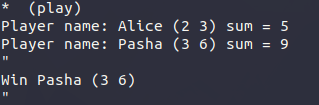
\includegraphics[width=0.5\textwidth]{img/2.png}
	% 		\caption{Результат работы 2.} }
	% \end{figure}

		
	% \begin{figure}[ht!]
	% 	\centering{
	% 		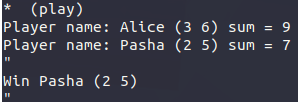
\includegraphics[width=0.5\textwidth]{img/3.png}
	% 		\caption{Результат работы 3.} }
	% \end{figure}

		
	% \begin{figure}[ht!]
	% 	\centering{
	% 		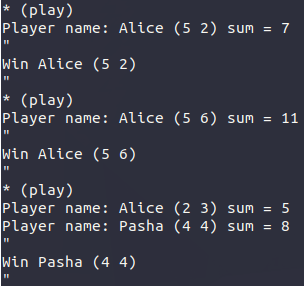
\includegraphics[width=0.5\textwidth]{img/4.png}
	% 		\caption{Результат работы 4.} }
	% \end{figure}

		
	% \begin{figure}[ht!]
	% 	\centering{
	% 		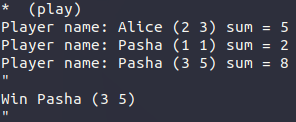
\includegraphics[width=0.5\textwidth]{img/5.png}
	% 		\caption{Результат работы 5.} }
	% \end{figure}
\end{task}



\newpage

\section*{Теоретическая часть}

\subsection*{Структуроразрушающие и не разрушающие структуру списка функции}

Функции для работы со списками делятся на две группы:

\begin{enumerate}
    \item Не разрушающие структуру. Если сохраняется возможность работать с исходными списками, значит функции не разрушают структуру.
    (Пример: append, reverse, length, subst ...)
    \item Разрушающие структуру. 
    Если после использования какой-то стандартной функции после ее работы теряется 
    возможность работы с теми списками, которые изначально были, значит их структура разрушилась. 
    Чаще всего такие функции начинаются в буквы 'n (Пример: nconc, nreverse, nsubst ...)
\end{enumerate}

\section*{Отличие в работе функции cons, list, append и в их результате}

\end{document}